
\section{Reihen\formelbuch{469, 1073}}

\subsection{Zahlenreihen\formelbuch{470}}
$ s_n = \sum\limits_{k=1}^{n} a_k \qquad $ ist eine (unendliche) Reihe. Sie ist die Folge von Partialsummen einer bestehenden Folge $a_n$.

\subsubsection{Konvergenz, Divergenz\formelbuch{471}}
Konvergiert die Reihe $< s_n >$ gegen die Summe $ s = \sum\limits_{k=1}^{\infty} a_k $ so ist sie konvergent. 
Existiert der GW nicht, so ist sie divergent.

\subsubsection{Konvergenzkriterien\formelbuch{462}}

\paragraph{Cauchy-Kriterium (Wurzelkriterium)} 
Wenn zu jedem $\varepsilon > 0$ ein Index $n_0$ existiert, so dass für alle $m > n > n_0$ gilt: \\
$\left| \sum\limits_{k=n}^m a_k \right| < \varepsilon$, dann konvergiert die Reihe, ansonsten divergiert sie.

\paragraph{lim = 0}
Wenn die Reihe $ \sum\limits_{n=1}^{\infty} a_n $ konvergent ist, so ist $\lim\limits_{n \to \infty} a_n = 0$. \hspace{2cm} Aber NICHT UMGEKEHRT!

\paragraph{Divergenz}
Ist $<a_n>$ divergent oder ist $\lim\limits_{n \to \infty} a_n \neq 0$, so ist die Reihe $ \sum\limits_{n=1}^{\infty} a_n $ divergent.

\paragraph{Majorantenkriterium\formelbuch{478}}
Ist die Reihe $ \sum\limits_{n=1}^{\infty} c_n $ konvergent, so konvergiert auch die Reihe $ \sum\limits_{n=1}^{\infty} |a_n|$ und somit auch
$\sum\limits_{n=1}^{\infty} a_n$ für $|a_n| \leq c_n$ (absolut).
Dies gilt auch für $|a_n| \leq c_n$ erst ab einer Stelle $n_0 \in \mathbb{N}$.\\
$\sum\limits_{n=1}^{m}a_k \leq |\sum\limits_{n=1}^{m}a_k| \leq \sum\limits_{n=1}^{m}|a_k| \leq \sum\limits_{n=1}^{m}c_n$

\paragraph{Minorantenkriterium}
Ist die Reihe $ \sum\limits_{n=1}^{\infty} d_n $ gegen $+\infty$ divergent, so gilt dies auch für die Reihe $ \sum\limits_{n=1}^{\infty} a_n $ 
bei $a_n \geq d_n$. \\ Dies gilt auch für $a_n \geq d_n$ erst ab einer Stelle $n_0 \in \mathbb{N}$. \\

\begin{tabular}{| p{4.5cm} | p{13.5cm} |}
	\hline
		\textbf{Reziprokkriterium} & 
		$ s = \sum\limits_{n=1}^{\infty} \frac{1}{n^\alpha} $ ist konvergent für $\alpha > 1$ und divergent für $\alpha \leq 1$.\\
	\hline
\end{tabular}

\begin{tabular}{| p{4.5cm} | p{8.5cm} | p{4.5cm} |}
	\hline
		\textbf{Quotientenkriterium}\formelbuch{473} &
		$ \lim\limits_{n \to \infty} \left|\frac{a_{n+1}}{a_n}\right| = \alpha $ der Reihe $ \sum\limits_{n=1}^{\infty} a_n$ &
		$\alpha < 1$ (aboslut) konvergent \\
	\cline{1-2}
		\textbf{Wurzelkriterium}\formelbuch{473} &
		$\lim\limits_{n \to \infty} \sqrt[n]{\left|a_n\right|} = \alpha $ der Reihe $ \sum\limits_{n=1}^{\infty} a_n$ &
		$\alpha = 1$ keine Aussage! \\
		&& $\alpha > 1$ divergent\\
	\hline
\end{tabular}

\begin{tabular}{| p{4.5cm} | p{13.5cm} |}
	\hline
		\textbf{Integralkriterium}\formelbuch{474} &
		$\int\limits_{1}^{\infty}f(x)dx$ konvergent $\Leftrightarrow \sum\limits_{n=1}^{\infty}f(n)$ konvergent. \\
		
		&Gilt nur, wenn $f$ auf $ [1, \infty) $ definiert und monoton fallend ($f'(x) \leq 0$) ist. \\
		&Zudem muss $ f(x) \geq 0 $ für alle $x \in [1, \infty)$ sein. \\
	\hline
		\textbf{Leibniz-Kriterium}\formelbuch{475} &
		Die \textbf{alternierende} Reihe $ \sum\limits_{n=1}^{\infty} a_n $ ist konvergent, wenn die Folge $<\left|a_n\right|>$ eine monoton fallende Nullfolge ($\lim\limits_{n \to \infty}
		\left|a_n\right| = 0 $) ist. Monotonie mittels Verhältnis ($ \left|\frac{a_{n+1}}{a_n}\right|$), Differenz ($ |a_{n+1}| - |a_n| \leq |a_{n+1}| $) oder \textit{vollständiger Induktion} beweisen.\\ 
	\hline
\end{tabular}
	
\paragraph{Abschätzung Restglied einer alternierenden konvergenten Reihe\formelbuch{471}}
	\qquad $|R_n| = |s-s_n|\leq |a_{n+1}|$



\subsubsection{Bedingte und Absolute Konvergenz\formelbuch{474}}
Eine Reihe $\sum\limits_{n=1}^{\infty}a_n$ heisst \textbf{absolut konvergent}, wenn die
Reihe $\sum\limits_{n=1}^{\infty}|a_n|$ konvergent ist.\\

\begin{tabular}{ p{4.5cm}  p{13.5cm}}
	\textbf{Bedingt Konvergent:} &  Eine Reihe hat durch Umordnen einen anderen Grenzwert oder wird divergent (somit nicht absolut konvergent).\\
	\textbf{Unbedingt Konvergent:} &  Durch Umordnen ändert sich der Grenzwert nicht.\\
\end{tabular}


\subsubsection{Produkt von absolut konvergenten Reihen\formelbuch{475}} 
Gegeben sei: $\sum a_n=a$, \quad $\sum b_n=b, \quad \sum c_n = (\sum a_n) \cdot (\sum b_n) = c \quad $ so ist
$ \quad c_n=\sum a_kb_{n-k+1} \quad $ und $ \quad c = a \cdot b $
	
\subsubsection{Geometrische Reihe}
Es sei $a_1\in\mathbb R$ und $q\in\mathbb R \backslash \{0;1\}$, dann erh"alt
man aus der geometrischen Folge $\langle a_k \rangle$ mit $a_k=a_1 \cdot
q^{k-1}$ die geometrische Reihe $\langle s_n \rangle$ mit
\textbf{$s_n= \sum\limits_{k=1}^{n} a_1 \cdot q^{k-1}=a_1 \cdot
\frac{1-q^n}{1-q}$\\}
\paragraph{Monotonie}
\begin{tabular}{ll}
$s_n \leq 0$&$\to$ (streng) monoton Fallend\\
$s_m \geq 0$&$\to$ (streng) monoton Steigend\\
$0 < q \leq 1$&$\to$ (streng) monoton Fallend\\
$0 < q \geq 1$&$\to$ (streng) monoton Stieigend\\
\end{tabular}

\subsubsection{Harmonische Reihe}
Aus der Folge $\langle a_k \rangle$ mit $a_k=\frac{1}{k}$ erhalten wir die
harmonisch Reihe mit $\langle s_n \rangle$ mit
\textbf{$s_n=\sum\limits_{k=1}^{n}
\frac{1}{k}=1+\frac{1}{2}+\frac{1}{3}+\dotsc+\frac{1}{n}$}
\subsubsection{Konvergenzkriterien}

Eine konvergente oder divergente Reihe bleibt konvergent oder divergent auch wenn man endlich viele Summanden entfernt!
Abschätzung Restglied = Fehlerabschätzung. \\

\subsection{Potenzreihen\formelbuch{481}}

\subsubsection{Definition\formelbuch{432}} 
Die Reihe $ \sum\limits_{n=0}^{\infty} a_n (x-x_0)^n $ heisst Potenzreihe mit Entwicklungspunkt $x_0$ und Koeffizienten $a_n$.

\begin{tabular}{lll}
\textbf{Geometrische Reihe\formelbuch{19}}
	& $a \cdot \sum\limits_{n=0}^{\infty} q^n = \frac{a}{1-q}$
	& $(|q| < 1) \qquad$ Beidseitiges $\int \quad\Rightarrow\quad a \cdot \sum\limits_{n=1}^{\infty} \frac{q^{n}}{n} = -a \cdot \ln{|1-q|} $ \\
\textbf{Binominalreihe\formelbuch{12}} 
	& $\sum\limits_{n=0}^\infty \binom{\alpha}{n} x^n = (1+x)^\alpha$
	& $x \in (-1,1)\qquad$ Binominalkoeff. $\binom{n}{k} = \frac{n!}{(n-k)!k!} $\\
\textbf{Taylor-Reihe\formelbuch{483}}
	& $ \sum\limits_{n=0}^{\infty} \frac{f^{(n)}(x_0)}{n!}\cdot(x-x_0)^n$
	& Taylor-Reihe von f bezüglich der Stelle $x_0$ \\
\textbf{E-Funktion}
	& \multicolumn{2}{l}{$e = \lim\limits_{n\to\infty} \left(1+\frac{1}{n}\right)^n = 
	\sum\limits_{k=0}^{\infty}{\frac{1}{k!}} = 1 + \frac{1}{1} + \frac{1}{1\cdot 2} +
	\frac{1}{1\cdot 2\cdot 3}  + \frac{1}{1\cdot 2\cdot 3\cdot4} + \cdots$} \\

	&$e^x = \sum\limits_{n=0}^{\infty}\frac{1}{n!} \cdot x^n$ &
	für $x_0 = 0$
\end{tabular}

\subsubsection{Konvergenz\formelbuch{481}}
Gegeben sei die Potenzreihe $ \sum\limits_{n=0}^{\infty} a_n x^n $ mit $ \lim\limits_{n \to \infty} \sqrt[n]{|a_n|} = a $ oder $\lim\limits_{n \to \infty} |\frac{a_{n+1}}{a_n}| = a$ \\
Für $ a=0 $ ist die Potenzreihe für alle $ x \in \mathbb{R} $ absolut konvergent. \\
Für $ a>0 $ ist die Potenzreihe für alle $x$ mit 
$	\left\{ 	
		\begin{array}{l} 
			|x| < \frac{1}{a} = r \Rightarrow \text{ absolut konvergent.} \\
			|x| > \frac{1}{a} = r \Rightarrow \text{ divergent.}
		\end{array} 
	\right. $ \\
Ist die Folge $<\sqrt[n]{|a_n|}>$ nicht beschränkt, so ist die Potenzreihe nur für $x=0$ konvergent.

\subsubsection{Abel's Theorem}
$ \sum\limits_{n=0}^{\infty}a_n \cdot r^n$ konvergent  $= \lim\limits_{x \uparrow r}f(x)$ (= Summe der Reihe) 

\subsubsection{Konvergenzradius\formelbuch{481}}
Jeder Potenzreihe kann ein Konvergenzradius $r$ zugeordnet werden. Wobei gilt $r = \frac{1}{a}$ mit $a = \lim\limits_{n \to \infty} \sqrt[n]{|a_n|} $. \\
Für $a = 0$ gilt $r = \infty$. Wenn a nicht exisitiert (Folge divergent) ist $r = 0$. \\
Berechnung mittels Quotientenkriterium: $ r = \lim\limits_{n \to \infty} \left| \frac{a_n}{a_{n+1}} \right| = \lim\limits_{n\to\infty} \frac{1}{\sqrt[n]{|a_n|}}$

\subsubsection{Differentiation}
Alle Potenzreihen mit einem $\rho > 0$ sind für alle $x \in (-\rho, \rho)$ beliebig oft (gliedweise) differenzierbar. \\
Der Potenzradius $\rho$ ist bei allen Ableitungen gleich demjenigen der Ursprungsfunktion. $\rho_{f} = \rho_{f^{(i)}}$.
$$ f(x) = \sum\limits_{n=0}^{\infty} a_n x^n  \qquad 
   f'(x) = \sum\limits_{n=1}^{\infty} n \cdot a_n x^{n-1 } \qquad 
   f''(x) = \sum\limits_{n=2}^{\infty} n(n-1) \cdot a_n x^{n-2} \qquad 
   f^{(i)}(x) = \sum\limits_{n=i}^{\infty} n(n-1)\cdot \ldots \cdot (n-i+1)\cdot a_n x^{n-i} $$ 
\textbf{Bemerkung:} Startwert ($n=0$) nur erhöhen, wenn bei $x^n, n$ negativ werden würde!
\subsubsection{Integration}
\paragraph{Unbestimmtes Integral}
$\int \sum\limits_{n=0}^{\infty} a_n x^n dx = 
\sum\limits_{n=0}^{\infty} a_n \int x^n dx = 
\sum\limits_{n=0}^{\infty} \frac{a_n}{n+1}\cdot x^{n+1} \qquad \text{ für alle } x \in (-\rho, \rho).$
\paragraph{Bestimmtes Integral}
$\int\limits_0^x \sum\limits_{n=0}^{\infty} a_n t^n dt = 
\sum\limits_{n=0}^{\infty} \frac{a_n}{n+1}\cdot x^{n+1} \qquad \text{ für alle } x \in (-\rho, \rho).$
\renewcommand{\arraystretch}{1.5}
\subsection{Grenzwerte von Reihen}

\begin{tabular}{| l | l | l | l |}
	\hline
		$\lim\limits_{n\to\infty}(1+\frac{x}{n})^n = e^x$ &
		$\lim\limits_{n\to\infty}(\sqrt[n]{a}) = 1$ ($a > 0$ und const.) &
		$\lim\limits_{n\to\infty}(\sqrt[n]{n}) = 1$ &
		$\lim\limits_{n\to\infty}(\sqrt[n]{n^a}) = 1$ ($a$ const.)\\
	\hline
		$\lim\limits_{n\to\infty}(\sqrt[n]{|p(n)|}) = 1$ ($p(n) \neq 0$) &
		$\lim\limits_{n\to\infty}(\frac{K}{n!}) = 0$ ($K$ const.) &
		$\lim\limits_{n\to\infty}(\sqrt[n]{n!}) = +\infty$ &
		$\lim\limits_{n\to\infty}(\sqrt[n]{\frac{K^n}{n!}}) = 0$ ($K > 0$ und const.)\\
	\hline
		$\lim\limits_{n\to\infty}(\frac{n}{\sqrt[n]{n!}}) = e$ &&&\\
	\hline		
\end{tabular}

\subsection{einige Reihen}

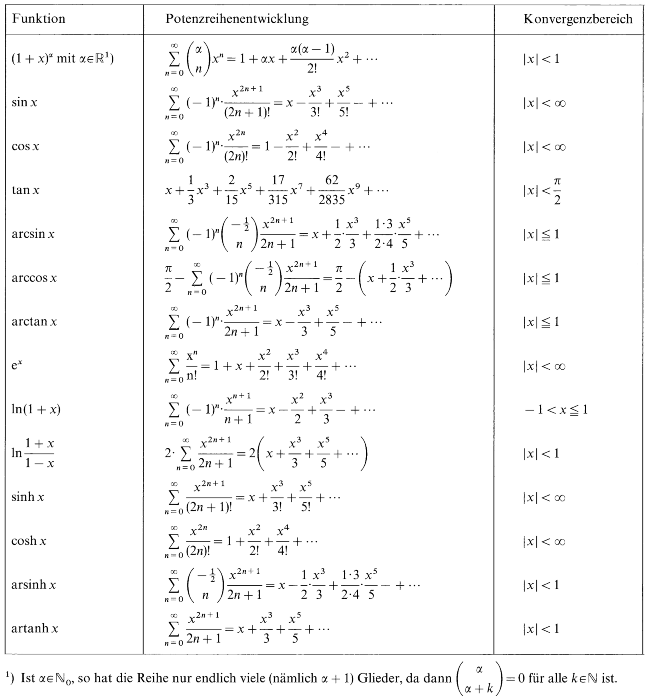
\includegraphics[height=17.0cm]{./bilder/reihen.png}

	Leibniz-Reihe: $ \sum\limits_{n=0}^{\infty} \frac{(-1)^n}{2^{n+1}} = 1-\frac{1}{3}+\frac{1}{5}-\frac{1}{7}+...+=\frac{\Pi}{4} $

	$\sum\limits_{n=1}^{\infty} \frac{1}{n} \rightarrow$ ist divergent \\
	$\sum\limits_{n=1}^{\infty} \frac{1}{n^2} \rightarrow$ absolut konvergent gegen 1 (beweisen mit Integralkriterium)

\renewcommand{\arraystretch}{1.2}
%%%%%%%%%%%%%%%%%%%%%%%%%%%%%%%%%%%%%%%%%%%%%%%%%%%%%%%%%%%%%%%%%%%%%%%%%%%%%%%%%%%%%%%%%%%%%%%%
%%%%%%%%%%%%%%%%%%%%%%%%%%%%%%%%%%%%%%%%%%%%%%%%%%%%%%%%%%%%%%%%%%%%%%%%%%%%%%%%%%%%%%%%%%%%%%%%
